\chapter{Implementando oVirt}
\label{sec:ovirt}

\section{Instalación del motor}
\label{sec:ovirt_install}

Una vez instalado el sistema operativo en el nodo de control (Fedora, RHEL, o CentOS 7)\footnote{Léase anexo para el proceso de instalación de CentOS}, hace falta actualizar los paquetes del sistema:

\begin{TMterminal}{}{}{Actualizando paquetes}
  yum -y update
\end{TMterminal}

El siguiente paso para instalar oVirt es subscribirnos a su repositorio. Instalar el siguiente RPM es similar a añadir un PPA en distribuciones basadas en Ubuntu en el hecho de que actualizaciones a éste paquete deberían aparecer al hacer más \texttt{yum update} en el futuro.

\begin{TMterminal}{}{}{Instalando oVirt}
  yum install http://plain.resources.ovirt.org/pub/yum-repo/ovirt-release35.rpm
  yum -y install ovirt-engine
\end{TMterminal}

Cuando el paquete se haya instalado, ejecutaremos el instalador del motor, que nos hará una serie de preguntas. El siguiente es un ejemplo del mismo instalador, con las respuestas por defecto envueltas entre corchetes \cite{ovirt}.

\begin{TMterminal}{}{}{Instalación del motor}
  engine-setup
[ INFO  ] Stage: Initializing
   [ INFO  ] Stage: Environment setup
           Configuration files: ['/etc/ovirt-engine-setup.conf.d/10-packaging.conf']
           Log file: /var/log/ovirt-engine/setup/ovirt-engine-setup-20140310163840.log
           Version: otopi-1.2.0_rc2 (otopi-1.2.0-0.7.rc2.fc19)
   [ INFO  ] Stage: Environment packages setup
   [ INFO  ] Stage: Programs detection
   [ INFO  ] Stage: Environment setup
   [ INFO  ] Stage: Environment customization
          
           --== PRODUCT OPTIONS ==--
           --== PACKAGES ==--
          
   [ INFO  ] Checking for product updates...
   [ INFO  ] No product updates found
      
           --== NETWORK CONFIGURATION ==--
          
           Host fully qualified DNS name of this server [server.name]: example.ovirt.org
           Setup can automatically configure the firewall on this system.
           Note: automatic configuration of the firewall may overwrite current settings.
           Do you want Setup to configure the firewall? (Yes, No) [Yes]:
   [ INFO  ] firewalld will be configured as firewall manager.
          
           --== DATABASE CONFIGURATION ==--
          
           Where is the Engine database located? (Local, Remote) [Local]: 
           Setup can configure the local postgresql server automatically for the engine to run. This may conflict with existing applications.
           Would you like Setup to automatically configure postgresql and create Engine database, or prefer to perform that manually? (Automatic, Manual) [Automatic]: 
          
           --== OVIRT ENGINE CONFIGURATION ==--
          
           Application mode (Both, Virt, Gluster) [Both]: 
           Default storage type: (NFS, FC, ISCSI, POSIXFS) [NFS]: 
           Engine admin password: 
           Confirm engine admin password: 
          
           --== PKI CONFIGURATION ==--
          
           Organization name for certificate [ovirt.org]: 
          
           --== APACHE CONFIGURATION ==--
          
           Setup can configure apache to use SSL using a certificate issued from the internal CA.
     
           Do you wish Setup to configure that, or prefer to perform that manually? (Automatic, Manual) [Automatic]: 
           Setup can configure the default page of the web server to present the application home page. This may conflict with existing applications.
           Do you wish to set the application as the default page of the web server? (Yes, No) [Yes]: 
          
           --== SYSTEM CONFIGURATION ==--
          
           Configure WebSocket Proxy on this machine? (Yes, No) [Yes]: 
           Configure an NFS share on this server to be used as an ISO Domain? (Yes, No) [Yes]: 
           Local ISO domain path [/var/lib/exports/iso-20140310143916]: 
           Local ISO domain ACL - note that the default will restrict access to example.ovirt.org only, for security reasons [example.ovirt.org(rw)]: 
           Local ISO domain name [ISO_DOMAIN]: 
          
           --== MISC CONFIGURATION ==--
     
           --== END OF CONFIGURATION ==--

        [ INFO  ] Stage: Setup validation
          
                    --== CONFIGURATION PREVIEW ==--
          
           Engine database name                    : engine
           Engine database secured connection      : False
           Engine database host                    : localhost
           Engine database user name               : engine
           Engine database host name validation    : False
           Engine database port                    : 5432
           NFS setup                               : True
           PKI organization                        : ovirt.org
           Application mode                        : both
           Firewall manager                        : firewalld
           Update Firewall                         : True
           Configure WebSocket Proxy               : True
           Host FQDN                               : example.ovirt.org
           NFS export ACL                          : 0.0.0.0/0.0.0.0(rw)
           NFS mount point                         : /var/lib/exports/iso-20140310143916
           Datacenter storage type                 : nfs
           Configure local Engine database         : True
           Set application as default page         : True
           Configure Apache SSL                    : True
           Please confirm installation settings (OK, Cancel) [OK]:   
   [ INFO  ] Stage: Transaction setup
   [ INFO  ] Stopping engine service
   [ INFO  ] Stopping websocket-proxy service
   [ INFO  ] Stage: Misc configuration
   [ INFO  ] Stage: Package installation
   [ INFO  ] Stage: Misc configuration
   [ INFO  ] Creating PostgreSQL 'engine' database
   [ INFO  ] Configuring PostgreSQL
   [ INFO  ] Creating Engine database schema
   [ INFO  ] Creating CA
   [ INFO  ] Configuring WebSocket Proxy
   [ INFO  ] Generating post install configuration file '/etc/ovirt-engine-setup.conf.d/20-setup-ovirt-post.conf'
   [ INFO  ] Stage: Transaction commit
   [ INFO  ] Stage: Closing up
          
           --== SUMMARY ==--
           `         SSH fingerprint: `<SSH_FINGERPRINT> `         Internal CA: `<CA_FINGERPRINT>
           Web access is enabled at: `             `[`http://example.ovirt.org:80/ovirt-engine`](http://example.ovirt.org:80/ovirt-engine) `             `[`https://example.ovirt.org:443/ovirt-engine`](https://example.ovirt.org:443/ovirt-engine)
           Please use the user "admin" and password specified in order to login into oVirt Engine
          
           --== END OF SUMMARY ==--
          
   [ INFO  ] Starting engine service
   [ INFO  ] Restarting httpd
   [ INFO  ] Restarting nfs services
   [ INFO  ] Generating answer file '/var/lib/ovirt-engine/setup/answers/20140310163837-setup.conf'
   [ INFO  ] Stage: Clean up
           Log file is located at /var/log/ovirt-engine/setup/ovirt-engine-setup-20140310163604.log
   [ INFO  ] Stage: Pre-termination
   [ INFO  ] Stage: Termination
   [ INFO  ] Execution of setup completed successfully
     
     **** Installation completed successfully ******
\end{TMterminal}

\bigskip

\begin{TMterminal}{}{}{Nota}
  Configuraré los \emph{exports} NFS a mano, así que omitiré la parte del instalador que configura un dominio ISO.
\end{TMterminal}

Una vez hecho ésto, ya estaremos listos para acceder a la interfaz web del motor, con la contraseña que le hemos dicho al instalador.

\section{Instalación de los Host}
\label{sec:host_inst}

A la hora de montar los hosts de virtualización, disponemos de varias opciones: podemos instalar el hipervisor propio de oVirt Node, que una vez configurado se añade automáticamente en el motor, o instalar el paquete encima de un CentOS o Fedora ya instalado. Ésta será la opción que documentaré.

Dicho ésto, para instalar el paquete, primero deberíamos asegurarnos que el sistema está actualizado:

\begin{TMterminal}{}{}{Actualizando paquetes}
  yum -y update
\end{TMterminal}

\bigskip

Y instalamos oVirt:

\begin{TMterminal}{}{}{Instalando paquetes}
  yum localinstall http://plain.resources.ovirt.org/pub/yum-repo/ovirt-release36.rpm
\end{TMterminal}

\bigskip

Cuando ya esté instalado, podemos añadirlo manualmente a oVirt, en la pestaña Hosts. Cuando cliquemos en \emph{New}, aparecerá el siguiente diálogo: \clearpage

\begin{figure}[h!]
  \centering
  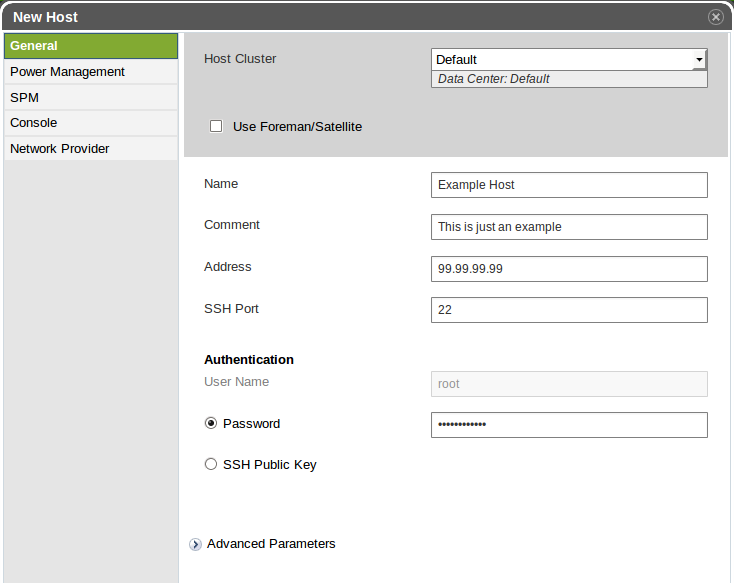
\includegraphics[scale=0.55]{ovirt_hostinst.png}
  \caption{\label{fig:ovirthostinst} Añadiendo el host}
\end{figure}

Una vez añadido, oVirt descargará e instalará ciertos paquetes. Podemos ver el progreso de ésta tarea en la parte inferior de la pantalla, en las pestañas Events y Tasks.

\section{Configuración del almacenamiento}
\label{sec:almacenamiento}

Como ya mencioné cuando describía la arquitectura de oVirt, el almacenamiento viene proporcionado por un sistema en red. Las opciones incluyen soluciones como GlusterFS, iSCSI, o FCP, pero nosotros usaremos NFS.\@ Hay que tener en cuenta, que el tipo de almacenamiento que se use debe coincidir con el tipo por defecto que se seleccionó en el instalador.

Entonces, para configurar los \emph{exports} que usaremos en oVirt, instalamos el servidor, y lo configuramos acordemente \footnote{Ésta configuración sirve sólo de ejemplo: léase la documentación de NFS}:

\begin{TMterminal}{}{}{Configurando NFS}
  yum -y install nfs-utils
  vi /etc/exports
---------------------------
/srv/ovirt/export  *(rw,sync,no_subtree_check,all_squash,anonuid=36,anongid=36)
/srv/ovirt/data    *(rw,sync,no_subtree_check,all_squash,anonuid=36,anongid=36)
/srv/ovirt/iso     *(rw,sync,no_subtree_check,all_squash,anonuid=36,anongid=36)
/usr/ovirt/disks   *(rw,sync,no_subtree_check,all_squash,anonuid=36,anongid=36)
\end{TMterminal}

Una vez hecho ésto, debemos añadirlos en el siguiente orden en la interfaz de administración web:

\begin{enumerate}
    \item Export
    \item Data
    \item iso
\end{enumerate}

\subsection{Cargando las ISOs}
\label{subsec:isos}

Cuando ya tenemos el almacenamiento en red configurado, una particularidad de oVirt es que no podemos abocar directamente al directorio /srv/ovirt/iso las imágenes de instalación, sino que debemos usar la herramienta \texttt{engine-iso-uploader} para subirlas al datacenter, y puedan ser usadas para posteriormente instalar sistemas operativos en las máquinas virtuales. A continuación muestro un ejemplo de dicho comando:

\begin{TMterminal}{}{}{Subiendo ISOs}
  engine-iso-uploader -i nombre_del_dominio_en_ovirt upload imagen.iso
\end{TMterminal}

\subsection{Creando los discos}
\label{subsec:creando_discos}

La creación de los discos puede hacerse tanto al momento de crear la máquina virtual, o cuando el usuario quiera. De todas maneras el proceso es el mismo, detallado en la siguiente captura: 

\begin{figure}[ht!]
  \centering
  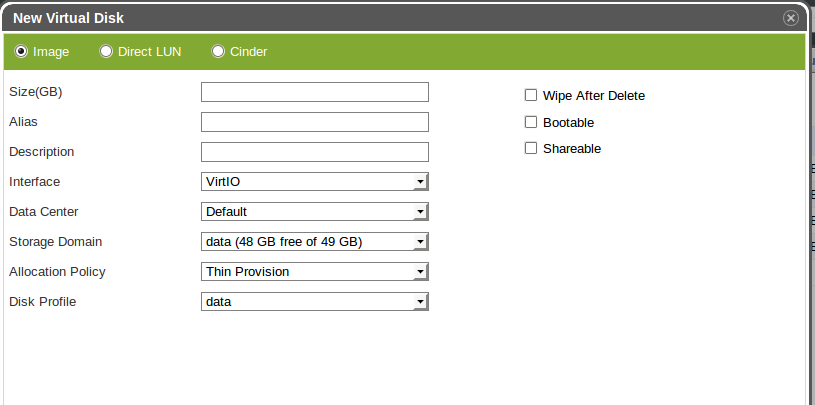
\includegraphics[scale=0.55]{ovirt_newdisk.png}
  \caption{\label{fig:create_disk} Creando discos}
\end{figure}
\clearpage

\subsection{Creando interfaces de red}
\label{subsec:creando_interfaces}

Antes de proceder finalmente a crear una máquina virtual, debemos crear la interfaz de red.

\begin{figure}[ht!]
  \centering
  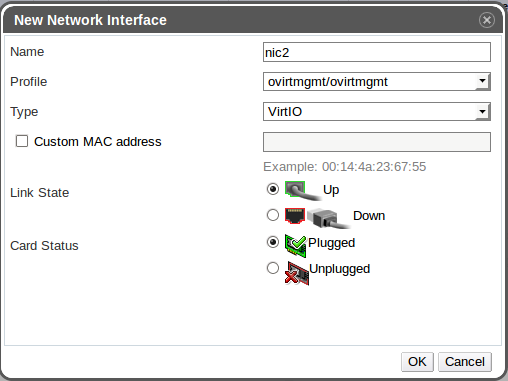
\includegraphics[scale=0.55]{ovirt_newnic.png}
  \caption{\label{fig:create_nic} Creando interfaces de red}
\end{figure}

Acorde a la captura, podemos escoger varios tipos de interfaces de red:

\begin{itemize}
    \item \textbf{VirtIO:\@ }La opción más rápida y ligera, si el sistema virtualizado lo soporta
    \item \textbf{Dos modelos de tarjetas físicas reales: }Su uso supone más \emph{overhead}, ya que tienen que virtualizarse las tarjetas por completo.
    \item \textbf{NIC Passthrough: }Otorga de forma exclusiva una interfaz de red de la máquina anfitriona al sistema virtualizado.
\end{itemize}

\clearpage

\section{Creando máquinas virtuales}
\label{sec:creando_vms}

La creación de las máquinas virtuales es bastante simple. Se puede acceder al diálogo de creación de máquinas virtuales mediante el menú Virtual Machines > New. Las siguientes capturas muestran algunas de las opciones de las que disponemos a la hora de crearlas:

\begin{figure}[ht!]
  \centering
  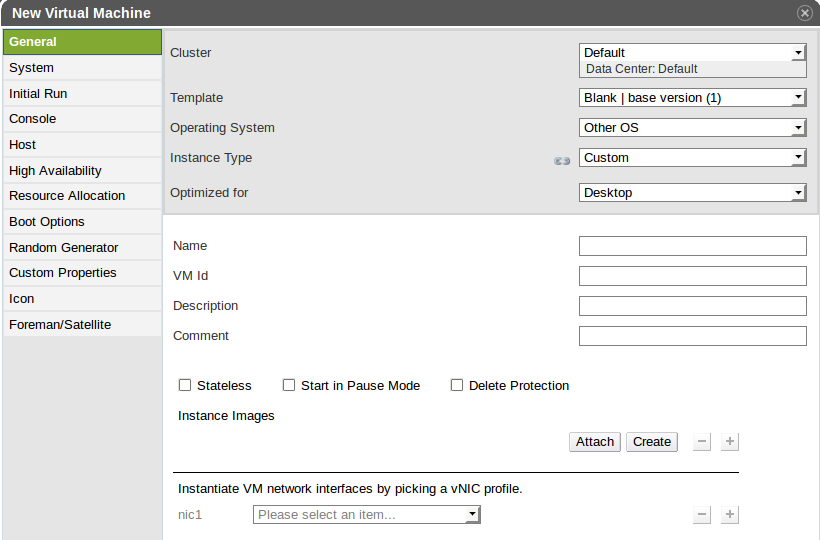
\includegraphics[scale=0.55]{ovirt_newvm.png}
  \caption{\label{fig:create_vms} Creando máquinas virtuales}
\end{figure}

\begin{figure}[ht!]
  \centering
  \frame{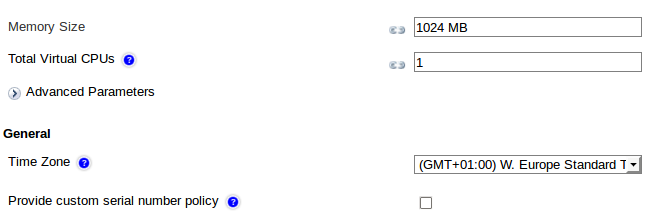
\includegraphics[scale=0.55]{ovirt_vm_system.png}}
  \caption{\label{fig:vmsys} Opciones de sistema}
\end{figure}

\begin{figure}[ht!]
  \centering
  \frame{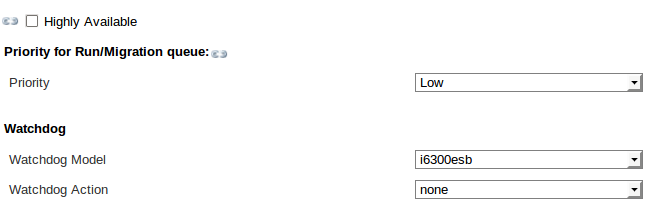
\includegraphics[scale=0.65]{ovirt_vms_ha.png}}
  \caption{\label{fig:vmha} Opciones de alta disponibilidad}
\end{figure}

\begin{figure}[ht!]
  \centering
  \frame{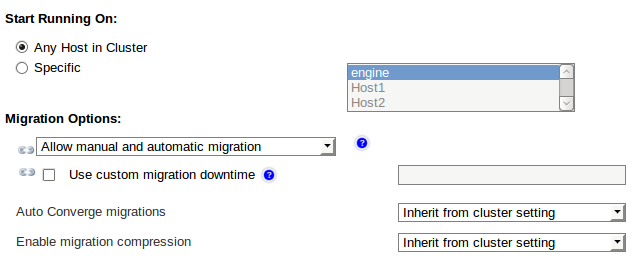
\includegraphics[scale=0.65]{ovirt_vm_host.png}}
  \caption{\label{fig:vmhost} Opciones de host}
\end{figure}

\begin{figure}[ht!]
  \centering
  \frame{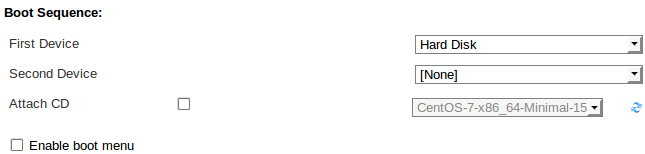
\includegraphics[scale=0.65]{ovirt_vm_boot.png}}
  \caption{\label{fig:vm_boot} Arranque}
\end{figure}

\clearpage
\subsection{oVirt Guest Agent}
\label{subsec:guestagent}

Una vez instaladas las máquinas, debemos instalar el oVirt Guest Agent. Ésta herramienta permite al sistema operativo virtualizado comunicarse con el nodo maestro, ofreciéndole información tal como la dirección IP, el \emph{FQDN} y estadísticas de uso de recursos. El proceso varía dependiendo del sistema operativo, pero a modo de ejemplo, el proceso en Ubuntu es el siguiente:

\begin{enumerate}
\item Editar el fichero \texttt{/etc/apt/sources.list.d/ovirt-guest-agent.list} añadiendo el siguiente contenido:

    \begin{TMterminal}{}{}{/etc/apt/sources.list.d/ovirt-guest-agent.list}
        deb http://download.opensuse.org/repositories/home:/evilissimo:/ubuntu:/14.04/xUbuntu_14.04/ /
    \end{TMterminal}

\item Añadir la \emph{Release key}:

    \begin{TMterminal}{}{}{Añadiendo la release key}
        wget http://download.opensuse.org/repositories/home:/evilissimo:/ubuntu:/14.04/xUbuntu_14.04//Release.key
        sudo apt-key add - < Release.key  
    \end{TMterminal}

\item Y finalmente, actualizamos las listas de software e instalamos el paquete:

    \begin{TMterminal}{}{}{Instalando}
        sudo apt-get update && sudo apt-get install ovirt-guest-agent
    \end{TMterminal}
\end{enumerate}

Una vez esté instalado, el servicio se autoejecutará en cada arranque de la máquina virtual. Si ahora vamos a la interfaz web, deberíamos ver la información de la siguiente manera:

\begin{figure}[ht!]
  \centering
  \hspace*{-1cm}
  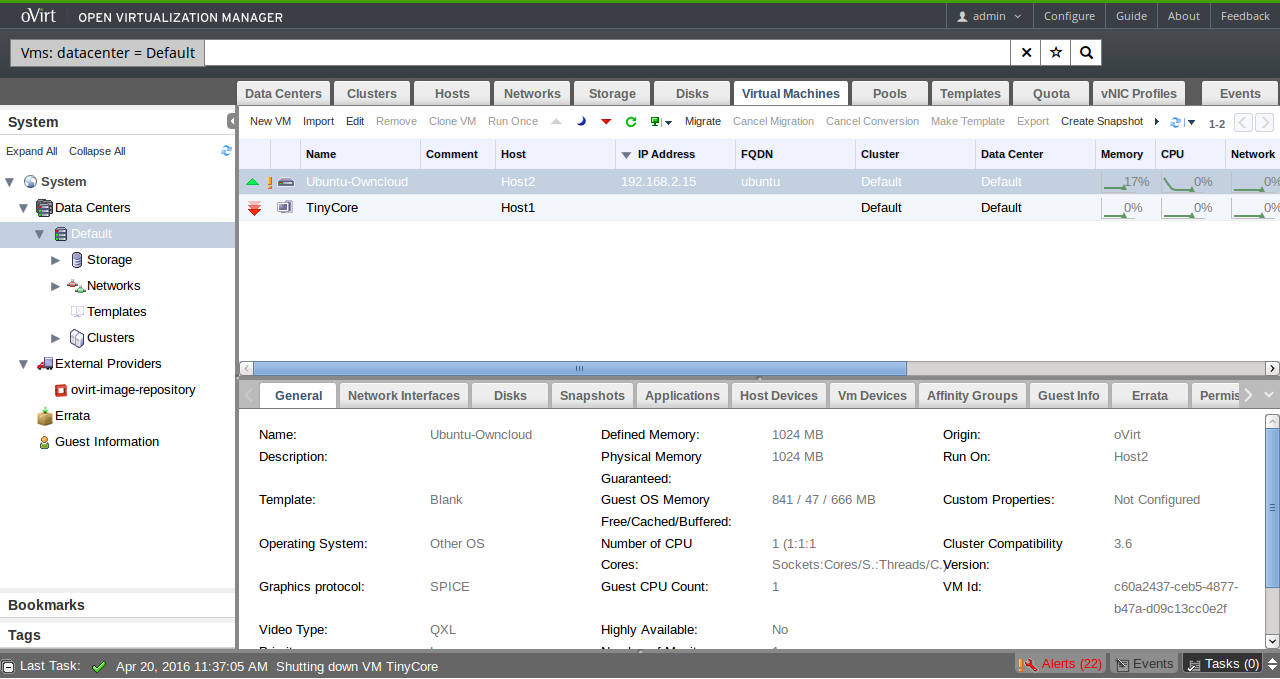
\includegraphics[scale=0.40]{ovirt-vms.png}
  \caption{\label{fig:listado_vms} Lista de máquinas virtuales}
\end{figure}











